% Options for packages loaded elsewhere
\PassOptionsToPackage{unicode}{hyperref}
\PassOptionsToPackage{hyphens}{url}
%
\documentclass[
]{book}
\usepackage{amsmath,amssymb}
\usepackage{lmodern}
\usepackage{ifxetex,ifluatex}
\ifnum 0\ifxetex 1\fi\ifluatex 1\fi=0 % if pdftex
  \usepackage[T1]{fontenc}
  \usepackage[utf8]{inputenc}
  \usepackage{textcomp} % provide euro and other symbols
\else % if luatex or xetex
  \usepackage{unicode-math}
  \defaultfontfeatures{Scale=MatchLowercase}
  \defaultfontfeatures[\rmfamily]{Ligatures=TeX,Scale=1}
\fi
% Use upquote if available, for straight quotes in verbatim environments
\IfFileExists{upquote.sty}{\usepackage{upquote}}{}
\IfFileExists{microtype.sty}{% use microtype if available
  \usepackage[]{microtype}
  \UseMicrotypeSet[protrusion]{basicmath} % disable protrusion for tt fonts
}{}
\makeatletter
\@ifundefined{KOMAClassName}{% if non-KOMA class
  \IfFileExists{parskip.sty}{%
    \usepackage{parskip}
  }{% else
    \setlength{\parindent}{0pt}
    \setlength{\parskip}{6pt plus 2pt minus 1pt}}
}{% if KOMA class
  \KOMAoptions{parskip=half}}
\makeatother
\usepackage{xcolor}
\IfFileExists{xurl.sty}{\usepackage{xurl}}{} % add URL line breaks if available
\IfFileExists{bookmark.sty}{\usepackage{bookmark}}{\usepackage{hyperref}}
\hypersetup{
  pdftitle={04-Resistance-surface},
  pdfauthor={Chris B},
  hidelinks,
  pdfcreator={LaTeX via pandoc}}
\urlstyle{same} % disable monospaced font for URLs
\usepackage{color}
\usepackage{fancyvrb}
\newcommand{\VerbBar}{|}
\newcommand{\VERB}{\Verb[commandchars=\\\{\}]}
\DefineVerbatimEnvironment{Highlighting}{Verbatim}{commandchars=\\\{\}}
% Add ',fontsize=\small' for more characters per line
\usepackage{framed}
\definecolor{shadecolor}{RGB}{248,248,248}
\newenvironment{Shaded}{\begin{snugshade}}{\end{snugshade}}
\newcommand{\AlertTok}[1]{\textcolor[rgb]{0.94,0.16,0.16}{#1}}
\newcommand{\AnnotationTok}[1]{\textcolor[rgb]{0.56,0.35,0.01}{\textbf{\textit{#1}}}}
\newcommand{\AttributeTok}[1]{\textcolor[rgb]{0.77,0.63,0.00}{#1}}
\newcommand{\BaseNTok}[1]{\textcolor[rgb]{0.00,0.00,0.81}{#1}}
\newcommand{\BuiltInTok}[1]{#1}
\newcommand{\CharTok}[1]{\textcolor[rgb]{0.31,0.60,0.02}{#1}}
\newcommand{\CommentTok}[1]{\textcolor[rgb]{0.56,0.35,0.01}{\textit{#1}}}
\newcommand{\CommentVarTok}[1]{\textcolor[rgb]{0.56,0.35,0.01}{\textbf{\textit{#1}}}}
\newcommand{\ConstantTok}[1]{\textcolor[rgb]{0.00,0.00,0.00}{#1}}
\newcommand{\ControlFlowTok}[1]{\textcolor[rgb]{0.13,0.29,0.53}{\textbf{#1}}}
\newcommand{\DataTypeTok}[1]{\textcolor[rgb]{0.13,0.29,0.53}{#1}}
\newcommand{\DecValTok}[1]{\textcolor[rgb]{0.00,0.00,0.81}{#1}}
\newcommand{\DocumentationTok}[1]{\textcolor[rgb]{0.56,0.35,0.01}{\textbf{\textit{#1}}}}
\newcommand{\ErrorTok}[1]{\textcolor[rgb]{0.64,0.00,0.00}{\textbf{#1}}}
\newcommand{\ExtensionTok}[1]{#1}
\newcommand{\FloatTok}[1]{\textcolor[rgb]{0.00,0.00,0.81}{#1}}
\newcommand{\FunctionTok}[1]{\textcolor[rgb]{0.00,0.00,0.00}{#1}}
\newcommand{\ImportTok}[1]{#1}
\newcommand{\InformationTok}[1]{\textcolor[rgb]{0.56,0.35,0.01}{\textbf{\textit{#1}}}}
\newcommand{\KeywordTok}[1]{\textcolor[rgb]{0.13,0.29,0.53}{\textbf{#1}}}
\newcommand{\NormalTok}[1]{#1}
\newcommand{\OperatorTok}[1]{\textcolor[rgb]{0.81,0.36,0.00}{\textbf{#1}}}
\newcommand{\OtherTok}[1]{\textcolor[rgb]{0.56,0.35,0.01}{#1}}
\newcommand{\PreprocessorTok}[1]{\textcolor[rgb]{0.56,0.35,0.01}{\textit{#1}}}
\newcommand{\RegionMarkerTok}[1]{#1}
\newcommand{\SpecialCharTok}[1]{\textcolor[rgb]{0.00,0.00,0.00}{#1}}
\newcommand{\SpecialStringTok}[1]{\textcolor[rgb]{0.31,0.60,0.02}{#1}}
\newcommand{\StringTok}[1]{\textcolor[rgb]{0.31,0.60,0.02}{#1}}
\newcommand{\VariableTok}[1]{\textcolor[rgb]{0.00,0.00,0.00}{#1}}
\newcommand{\VerbatimStringTok}[1]{\textcolor[rgb]{0.31,0.60,0.02}{#1}}
\newcommand{\WarningTok}[1]{\textcolor[rgb]{0.56,0.35,0.01}{\textbf{\textit{#1}}}}
\usepackage{longtable,booktabs,array}
\usepackage{calc} % for calculating minipage widths
% Correct order of tables after \paragraph or \subparagraph
\usepackage{etoolbox}
\makeatletter
\patchcmd\longtable{\par}{\if@noskipsec\mbox{}\fi\par}{}{}
\makeatother
% Allow footnotes in longtable head/foot
\IfFileExists{footnotehyper.sty}{\usepackage{footnotehyper}}{\usepackage{footnote}}
\makesavenoteenv{longtable}
\usepackage{graphicx}
\makeatletter
\def\maxwidth{\ifdim\Gin@nat@width>\linewidth\linewidth\else\Gin@nat@width\fi}
\def\maxheight{\ifdim\Gin@nat@height>\textheight\textheight\else\Gin@nat@height\fi}
\makeatother
% Scale images if necessary, so that they will not overflow the page
% margins by default, and it is still possible to overwrite the defaults
% using explicit options in \includegraphics[width, height, ...]{}
\setkeys{Gin}{width=\maxwidth,height=\maxheight,keepaspectratio}
% Set default figure placement to htbp
\makeatletter
\def\fps@figure{htbp}
\makeatother
\setlength{\emergencystretch}{3em} % prevent overfull lines
\providecommand{\tightlist}{%
  \setlength{\itemsep}{0pt}\setlength{\parskip}{0pt}}
\setcounter{secnumdepth}{5}
\usepackage{booktabs}
\usepackage{amsthm}
\makeatletter
\def\thm@space@setup{%
  \thm@preskip=8pt plus 2pt minus 4pt
  \thm@postskip=\thm@preskip
}
\makeatother
\usepackage{booktabs}
\usepackage{longtable}
\usepackage{array}
\usepackage{multirow}
\usepackage{wrapfig}
\usepackage{float}
\usepackage{colortbl}
\usepackage{pdflscape}
\usepackage{tabu}
\usepackage{threeparttable}
\usepackage{threeparttablex}
\usepackage[normalem]{ulem}
\usepackage{makecell}
\usepackage{xcolor}
\ifluatex
  \usepackage{selnolig}  % disable illegal ligatures
\fi
\usepackage[]{natbib}
\bibliographystyle{apalike}

\title{04-Resistance-surface}
\usepackage{etoolbox}
\makeatletter
\providecommand{\subtitle}[1]{% add subtitle to \maketitle
  \apptocmd{\@title}{\par {\large #1 \par}}{}{}
}
\makeatother
\subtitle{Final Report}
\author{Chris B}
\date{27/04/2022}

\begin{document}
\maketitle

{
\setcounter{tocdepth}{1}
\tableofcontents
}
\hypertarget{prerequisites}{%
\chapter{Prerequisites}\label{prerequisites}}

All of the data and analyses contained within this document are available within the project \href{https://drive.google.com/drive/u/0/folders/16WO_xH6B66D0dqyfeISHEB0mfU9cWWZg}{Google Drive folder}. In order to gain acess to the folder (as it is not public), please email Christopher Beirne \href{mailto:c.w.beirne@gmail.com}{\nolinkurl{c.w.beirne@gmail.com}}.

This is a \emph{sample} book written in \textbf{Markdown}. You can use anything that Pandoc's Markdown supports, e.g., a math equation \(a^2 + b^2 = c^2\).

The \textbf{bookdown} package can be installed from CRAN or Github:

\begin{Shaded}
\begin{Highlighting}[]
\FunctionTok{install.packages}\NormalTok{(}\StringTok{"bookdown"}\NormalTok{)}
\CommentTok{\# or the development version}
\CommentTok{\# devtools::install\_github("rstudio/bookdown")}
\end{Highlighting}
\end{Shaded}

Remember each Rmd file contains one and only one chapter, and a chapter is defined by the first-level heading \texttt{\#}.

To compile this example to PDF, you need XeLaTeX. You are recommended to install TinyTeX (which includes XeLaTeX): \url{https://yihui.name/tinytex/}.

\hypertarget{intro}{%
\chapter{Introduction}\label{intro}}

\hypertarget{summary}{%
\section{Summary}\label{summary}}

Mountain ranges constitute biodiversity hotspots and their importance only grows as lowland species shift their ranges in elevation in response to climate change. Protecting gradients which connect low to high elevation habitats are thus essential to preserving future biodiversity. However, most of the world's mountain ranges are narrowly protected and lack the elevational distributions needed to preserve biodiversity. We map the connectivity and protected status of elevational gradients from oceans to mountain ranges in mainland central america to reveal where connectivity between protected areas and important habitats is needed and may be optimized.

\begin{Shaded}
\begin{Highlighting}[]
\CommentTok{\# NOPTES FOR THE INTRO}

\DocumentationTok{\#\# Justification:}


\NormalTok{For the connectivity evaluation, our aim was to identify broad regions of habitat that have the}
\NormalTok{potential to facilitate the movement of multiple species and maintain ecological processes.}


\NormalTok{Land}\SpecialCharTok{{-}}\NormalTok{use and land}\SpecialCharTok{{-}}\NormalTok{cover changes have impacted the ability of many natural ecosystems to provide ecosystem goods and services }\ControlFlowTok{for}\NormalTok{ an ever}\SpecialCharTok{{-}}\NormalTok{growing human population. This often has unintended consequences that may threaten biodiversity and ecosystem health.}





\NormalTok{ In the context of multi}\SpecialCharTok{{-}}\NormalTok{functional land}\SpecialCharTok{{-}}\NormalTok{use planning, there is growing interest }\ControlFlowTok{in}\NormalTok{ species}\SpecialCharTok{{-}}\NormalTok{agnostic approaches, modelling connectivity as a }\ControlFlowTok{function}\NormalTok{ of human landscape modification. }



\SpecialCharTok{**}\NormalTok{Elevational gradients}\SpecialCharTok{**}

\NormalTok{From}\SpecialCharTok{:}\NormalTok{ Elsen PR, Monahan WB, Merenlender }\FunctionTok{AM}\NormalTok{ (}\DecValTok{2018}\NormalTok{) Global patterns of protection of elevational gradients }\ControlFlowTok{in}\NormalTok{ mountain ranges. Proc Natl Acad Sci U S A }\DecValTok{115}\SpecialCharTok{:}\NormalTok{6004–}\FloatTok{6009.}\NormalTok{ https}\SpecialCharTok{:}\ErrorTok{//}\NormalTok{doi.org}\SpecialCharTok{/}\FloatTok{10.1073}\SpecialCharTok{/}\NormalTok{pnas}\FloatTok{.1720141115}
\NormalTok{      This paper assess the within park elevational covergae. This goes a step further through analysisng the between park structural connectivity between reefs and ridges. They state}\SpecialCharTok{:} \StringTok{". Ensuring conserva{-}tion outcomes for PAs with lower IUCN designations as well asstrategically placing PAs to better represent and connect elevationalgradients will enhance ecological representation and facilitate spe{-}cies range shifts under climate change."} \StringTok{"  Enhancing pro{-}tection along elevational gradients may be particularly important, in mitigating biodiversity loss as climate change is projected tosimultaneously alter elevational distributions of agriculture (16),human populations (17), and natural resources (18). Despite ageneral understanding of the importance of protecting elevationalgradients for the maintenance of ecological and evolutionaryprocesses, we lack knowledge of where and how well elevationalgradients are protected at broad geographic scales."}\NormalTok{ WOW}\SpecialCharTok{!}



\NormalTok{Key assumptions}\SpecialCharTok{:}

\NormalTok{We presume throughout that}\SpecialCharTok{:}

\NormalTok{ The organism }\ControlFlowTok{in}\NormalTok{ question is on average minimizing its costs when moving through this matrix }\SpecialCharTok{{-}}\NormalTok{ an assumption possibly appropriate }\ControlFlowTok{for}\NormalTok{ terrestrial animals, and terrestrial animal}\SpecialCharTok{{-}}\NormalTok{dispersed plants. Other animals will require different approaches.}

\NormalTok{structural connectivity focuses only on landscape }\FunctionTok{characteristics}\NormalTok{ (e.g., movement corridors, barriers),}


\NormalTok{NOTE }\SpecialCharTok{{-}}\NormalTok{ from corridorsdesign }\SpecialCharTok{{-}} \StringTok{"Our methods, together with the CorridorDesigner ArcGIS tools, are best suited for designing corridors in a heterogenous landscape at a regional (e.g. 2 {-} 500 km long) scale."}

\NormalTok{The best way to conduct this may be through using the graph apporach to identify key least cost paths }\OtherTok{{-}\textgreater{}}\NormalTok{ then exploding those with circuitscape into finer detail.}


\DocumentationTok{\#\# GREAT OVERVIEW: https://rdrr.io/cran/gdistance/f/vignettes/Overview.Rmd }


\NormalTok{https}\SpecialCharTok{:}\ErrorTok{//}\NormalTok{onlinelibrary.wiley.com}\SpecialCharTok{/}\NormalTok{doi}\SpecialCharTok{/}\FloatTok{10.1111}\SpecialCharTok{/}\NormalTok{geb}\FloatTok{.13456} 



\NormalTok{Key tools }\ControlFlowTok{for}\NormalTok{ further readings}\SpecialCharTok{:}

\NormalTok{http}\SpecialCharTok{:}\ErrorTok{//}\NormalTok{www.corridordesign.org}\SpecialCharTok{/}


\DocumentationTok{\#\# Types of Connectivity {-} structural is important in this context}

\NormalTok{From }\StringTok{"Marrec R, Abdel Moniem HE, Iravani M, et al (2020) Conceptual framework and uncertainty analysis for large{-}scale, species{-}agnostic modelling of landscape connectivity across Alberta, Canada. Sci Rep 10:1–14. https://doi.org/10.1038/s41598{-}020{-}63545{-}z"}

\StringTok{"Natural ecosystems offer habitat for many species, and human landscape modification typically involves habitat loss as well as the breaking up of continuous habitats into smaller remnant patches (fragmentation)9,10. Consequently, landscapes may lose connectivity, i.e., the degree to which they facilitate movement of organisms and their genes among patches11,12. Landscape connectivity can be quantified in three ways: structural landscape connectivity, potential functional connectivity, and actual functional connectivity13. Structural landscape connectivity can be determined from physical attributes, based on maps alone without reference to organismal movement behaviour. Potential functional connectivity relies on a set of assumptions on organismal movement behaviour to implement an organism perspective, e.g. by mapping a species’ habitat and setting a dispersal threshold. In contrast, actual functional connectivity refers to observed data (e.g., patch occupancy, radio tracking, mark{-}recapture, or molecular genetic data) that reflect actual rates of the exchange of individuals (or their genes) and may be used to test models of structural or potential functional connectivity"}

\StringTok{"We argue that a species{-}agnostic approach is conceptually better suited for integrating landscape connectivity into land{-}use planning, whereas a focal{-}species approach is better suited for conservation management (Fig. 1). Understanding the difference between these perspectives can help clarify conceptual differences, guide researchers in making decisions about how to model connectivity, and inform practitioners about the potential and limitations of resulting maps. Conservation is often based on focal species, e.g., in species{-}at{-}risk management, where it is paramount to adopt an organism perspective60 to define critical habitat and to consider the organism’s ability to move between habitat patches. This will result in a model of potential functional connectivity for the specific organism of interest, and a multi{-}species model can be derived by overlaying models for a representative suite of species10,22. In contrast, land{-}use planning focuses on the sustainable development of multi{-}functional landscapes. In this human{-}centred perspective, land parcel ownership and administrative boundaries define the relevant spatial scale and the degree to which landscape development can be influenced by policy, which in the case of Alberta includes the introduction of ecosystem services and biodiversity markets that play a major role in balancing environmental considerations with socio{-}economic drivers59. Regarding landscape connectivity, the focus thus lies on how human landscape alteration affects the connectivity of the remaining natural heritage system and how to compare the expected effect of local development alternatives on larger{-}scale connectivity. This focus is highly compatible with the modelling of connectivity based on human modification, which will result in a model of structural landscape connectivity."}
\end{Highlighting}
\end{Shaded}

\hypertarget{data-assembly}{%
\chapter{Data assembly}\label{data-assembly}}

The following chapter details how we determined the area of interest and where we acquired the data products to be used in the connectivity analyses. We include justification of data sources where appropriate.

\hypertarget{define-the-focal-area}{%
\section{Define the focal area}\label{define-the-focal-area}}

This project focuses on the area covered by the Mesoamerican Biological Corridor \href{https://en.wikipedia.org/wiki/Mesoamerican_Biological_Corridor}{MBC}, which spans most of mainland central America. This excludes islands in central America and the Caribbean, as these will likely need a differing set of ridge-to-reef definitions. We also exclude Mexico.

The full focal area spans:

\includegraphics{bookdown-demo_files/figure-latex/unnamed-chunk-8-1.pdf}

Below we show the exclusion of surrounding islands:

\includegraphics{bookdown-demo_files/figure-latex/unnamed-chunk-10-1.pdf}

For an up to date assessment of the Mesoamerican Biological Corridor in Panama alone see:

\href{https://movementecologyjournal.biomedcentral.com/articles/10.1186/s40462-019-0186-0}{Meyer, N. F., Moreno, R., Reyna-Hurtado, R., Signer, J., \& Balkenhol, N. (2020). Towards the restoration of the Mesoamerican Biological Corridor for large mammals in Panama: comparing multi-species occupancy to movement models. Movement ecology, 8(1), 1-14.}

\hypertarget{data-products}{%
\section{Data products}\label{data-products}}

\hypertarget{protected-areas}{%
\subsection{Protected areas}\label{protected-areas}}

Shape files for protected areas were downloaded from the Protected Planet database. We buffered the area of interest by 10km, then excluded any protected ares which fell outside of that zone. This means marine protected areas \textgreater10km from the shore are not considered. There are two broad types of park National and International designations (and many further subdivisions not considered here).

\textbf{REVIEW POINT} What should we prioritize? Or should we consider both? international parks are not separate from ``national'' parks, there is overlap. I will start by only considering ``national'' designations.

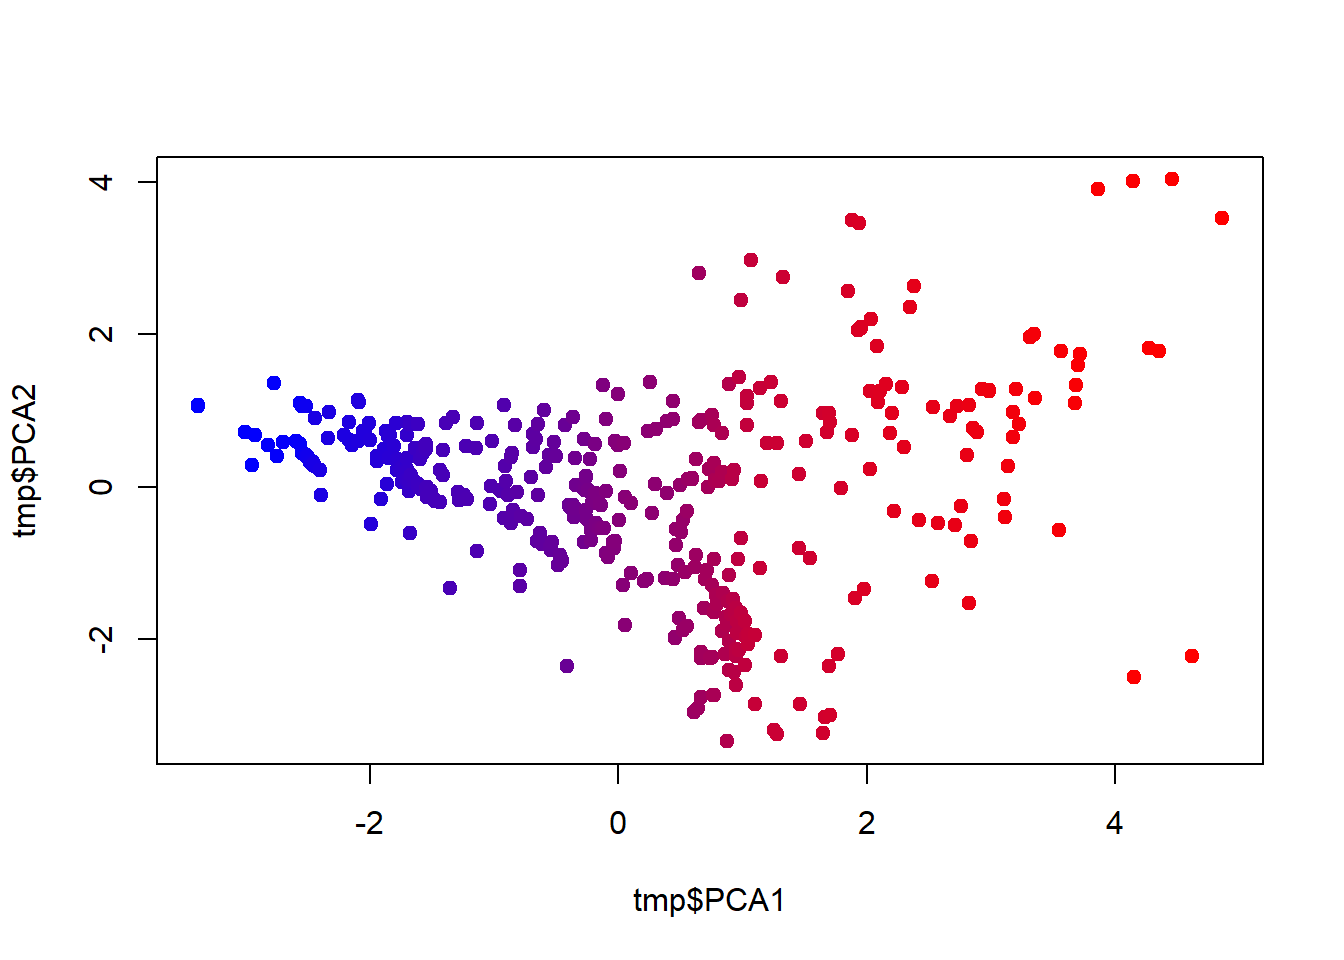
\includegraphics{bookdown-demo_files/figure-latex/unnamed-chunk-13-1.pdf}

Data source: UNEP-WCMC and IUCN (year), Protected Planet: The World Database on Protected Areas (WDPA) {[}February 2022{]}, Cambridge, UK: UNEP-WCMC and IUCN Available at: \href{www.protectedplanet.net}{Protected Planet}.

\hypertarget{types-of-protected-area}{%
\subsubsection{Types of protected area}\label{types-of-protected-area}}

The World Database on Protected Areas (WDPA) is the most up-to-date and complete source of information on protected areas, updated monthly with submissions from governments, non-governmental organizations, landowners, and communities. It is managed by the United Nations Environment Programme's World Conservation Monitoring Centre (UNEP-WCMC) with support from IUCN and its World Commission on Protected Areas (WCPA). This dataset includes the following number of terrestrial and marine protected areas:

\begin{table}
\centering
\begin{tabular}[t]{l|r}
\hline
Type & Freq\\
\hline
Terrestrial & 962\\
\hline
Marine & 112\\
\hline
\end{tabular}
\end{table}

There are also a myriad of different protection designations:

\begin{table}
\centering
\begin{tabular}[t]{l|r}
\hline
Type & Freq\\
\hline
Archaeological Reserve & 13\\
\hline
Area de Manejo de Hábitat & 1\\
\hline
Área de Manejo de Hábitat & 7\\
\hline
Area de Manejo de Hábitat/Especies & 7\\
\hline
Área de Manejo de Hábitat/Especies & 1\\
\hline
Área de Protección de Flora y Fauna & 2\\
\hline
Área de Protección y Restauración & 8\\
\hline
Área de Recursos Manejados & 2\\
\hline
Area de Uso Multiple & 4\\
\hline
Area de Uso Múltiple & 5\\
\hline
Área de Uso Múltiple & 2\\
\hline
Área Destinada Voluntariamente a la Conservación & 4\\
\hline
Area Marina de Manejo & 3\\
\hline
Área Natural & 62\\
\hline
Área Natural Protegida & 83\\
\hline
Área Natural Protegida Privada & 2\\
\hline
Área Productora de Agua & 2\\
\hline
Área Protegida con Recursos Manejados & 5\\
\hline
Área Recreativa & 2\\
\hline
Área Silvestre & 2\\
\hline
Biotopo Protegido & 6\\
\hline
Bosque Protector & 2\\
\hline
Bosque Protector y Paisaje Protegido & 1\\
\hline
Burdon Canal Nature Reserve & 1\\
\hline
Cockscomb Basin Wildlife Sanctuary & 1\\
\hline
Conservation Easement & 1\\
\hline
Corredor Biológico & 1\\
\hline
Crooked Tree Wildlife Sanctuary & 1\\
\hline
Forest Reserve & 16\\
\hline
Hol Chan & 1\\
\hline
Humedal & 12\\
\hline
Jardín Botánico y Centro de Investigación & 1\\
\hline
Labouring Creek Jaguar Corridor Wildlife Sanctuary & 1\\
\hline
Mangrove Reserve & 1\\
\hline
Monumento Cultural & 8\\
\hline
Monumento Historico & 1\\
\hline
Monumento Nacional & 3\\
\hline
Monumento Natural & 8\\
\hline
Monumento Natural Marino & 1\\
\hline
Mountain Pine Ridge Forest Reserve & 1\\
\hline
National Park & 16\\
\hline
Natural Monument & 3\\
\hline
Nature Reserve & 3\\
\hline
Nohoch Cheen Archaeological Reserve & 1\\
\hline
Paisaje Protegido & 4\\
\hline
Paisaje Terrestre Protegido & 15\\
\hline
Parque Ecológico & 1\\
\hline
Parque Nacional & 98\\
\hline
Parque Nacional Marino & 2\\
\hline
Parque Nacional Natural & 1\\
\hline
Parque Recreativo Natural Municipal & 1\\
\hline
Parque Regional & 1\\
\hline
Parque Regional Municipal & 76\\
\hline
Parque Regional y Área Natural Recreativa & 1\\
\hline
Port Honduras Marine Reserve & 1\\
\hline
Private Reserve & 8\\
\hline
Public Reserve & 5\\
\hline
Ramsar Site, Wetland of International Importance & 26\\
\hline
Refugio de Vida Silvestre & 37\\
\hline
Refugio Nacional de Vida Silvestre & 49\\
\hline
Reserva Antropológica y Forestal & 2\\
\hline
Reserva Biologica & 8\\
\hline
Reserva Biológica & 16\\
\hline
Reserva Biologica Marina & 1\\
\hline
Reserva Biósfera & 2\\
\hline
Reserva de la Biosfera & 8\\
\hline
Reserva de la Biósfera & 5\\
\hline
Reserva de Recursos & 1\\
\hline
Reserva de Recursos Genéticos & 2\\
\hline
Reserva de Uso Multiple & 1\\
\hline
Reserva Forestal & 16\\
\hline
Reserva Forestal Municipal & 2\\
\hline
Reserva Forestal Protectora de Manantiales & 1\\
\hline
Reserva Hídrica & 3\\
\hline
Reserva Hídrica y Forestal & 1\\
\hline
Reserva Hidrológica & 3\\
\hline
Reserva Natural & 53\\
\hline
Reserva Natural Absoluta & 2\\
\hline
Reserva Natural de la Sociedad Civil & 3\\
\hline
Reserva Natural Privada & 183\\
\hline
Reserva Protectora de Manantiales & 1\\
\hline
Reservas Forestales Protectoras Nacionales & 1\\
\hline
Reservas Naturales Privadas & 13\\
\hline
Sin Categoría Definida & 3\\
\hline
Sin definir & 1\\
\hline
Sitio Ramsar, Humedal de Importancia Internacional & 11\\
\hline
South Water Caye Marine Reserve & 1\\
\hline
Specially Protected Area (Cartagena Convention) & 1\\
\hline
UNESCO-MAB Biosphere Reserve & 12\\
\hline
Wildlife Sanctuary & 5\\
\hline
World Heritage Site (natural or mixed) & 9\\
\hline
Zona de Protección Hidrológica & 1\\
\hline
Zona de Reserva Ecológica & 2\\
\hline
Zona de Veda Definitiva & 30\\
\hline
Zona Protectora & 32\\
\hline
Zona Sujeta a Conservación Ecológica & 4\\
\hline
\end{tabular}
\end{table}

\hypertarget{marine-protected-areas}{%
\subsubsection{Marine protected areas}\label{marine-protected-areas}}

We may want to use marine protected areas as our focal nodes. Note - not all of these protected areas are fully marine. Some span land to sea.

\includegraphics{bookdown-demo_files/figure-latex/unnamed-chunk-16-1.pdf}

\textbf{REVIEW POINT} How effective are these protected areas? Are they all valid to include?

\hypertarget{elevation}{%
\subsection{Elevation}\label{elevation}}

We downloaded the elevation of the area of interest using SRTM Digital Elevation Data Version 4. The Shuttle Radar Topography Mission (SRTM) digital elevation dataset was originally produced to provide consistent, high-quality elevation data at near global scope.

\includegraphics{bookdown-demo_files/figure-latex/unnamed-chunk-18-1.pdf}

Data source: \href{https://srtm.csi.cgiar.org}{Jarvis, A., H.I. Reuter, A. Nelson, E. Guevara. 2008. Hole-filled SRTM for the globe Version 4, available from the CGIAR-CSI SRTM 90m Database}.

\hypertarget{forest-cover-current}{%
\subsection{Forest cover (current)}\label{forest-cover-current}}

To get a layer reflecting current forest cover we use the Hansen Global forest Change index. These reflect results from time-series analysis of Landsat images in characterizing global forest extent and change.

\includegraphics{bookdown-demo_files/figure-latex/unnamed-chunk-20-1.pdf}

Possible future data incorporation:

Current (and future) coarse vegetation types can also be obtained from this \href{https://www.nature.com/articles/s42003-021-02359-9}{Baumbach, L., Warren, D. L., Yousefpour, R., \& Hanewinkel, M. (2021). Climate change may induce connectivity loss and mountaintop extinction in Central American forests. Communications Biology, 4(1), 1-12.}

For an example approaches in modelling connectivity in the future (beyond the remit of this contract) see: \href{https://conbio.onlinelibrary.wiley.com/doi/epdf/10.1111/cobi.13904}{Mozelewski, T. G., Robbins, Z. J., Scheller, R. M., \& Mozelewski, T. G. (2022). Forecasting the influence of conservation strategies on landscape connectivity. Conservation Biology}

\hypertarget{forest-biomass}{%
\subsection{Forest biomass}\label{forest-biomass}}

We obtained above ground biomass from \href{https://doi.org/10.1038/s41597-020-0444-4}{Spawn, S.A., Sullivan, C.C., Lark, T.J. et al.~Harmonized global maps of above and belowground biomass carbon density in the year 2010. Sci Data 7, 112 (2020)}. This dataset provides temporally consistent and harmonized global maps of above-ground and below-ground biomass carbon density for the year 2010 at a 300-m spatial resolution.

\includegraphics{bookdown-demo_files/figure-latex/unnamed-chunk-22-1.pdf}

\hypertarget{forest-height}{%
\subsection{Forest height}\label{forest-height}}

For forest height we use the global 2005 dataset representing global tree heights based on a fusion of spaceborne-lidar data (2005) from the Geoscience Laser Altimeter System (GLAS) and ancillary geospatial data. See Simard et al.~(2011) for details.

\href{https://agupubs.onlinelibrary.wiley.com/doi/10.1029/2011JG001708}{Simard, M., Pinto, N., Fisher, J., Baccini, A. 2011. Mapping forest canopy height globally with spaceborne lidar. Journal of Geophysical Research. 116: G04021}

\includegraphics{bookdown-demo_files/figure-latex/unnamed-chunk-24-1.pdf}

\hypertarget{mangrove-cover-current}{%
\subsection{Mangrove cover (current)}\label{mangrove-cover-current}}

Mangrove data is taken from the {[}USGS: Global Distribution of Mangroves{]} (\url{https://data.unep-wcmc.org/datasets/4}).

\includegraphics{bookdown-demo_files/figure-latex/unnamed-chunk-26-1.pdf}

Citation:
Giri C, Ochieng E, Tieszen LL, Zhu Z, Singh A, Loveland T, Masek J, Duke N (2011). Status and distribution of mangrove forests of the world using earth observation satellite data (version 1.4, updated by UNEP-WCMC). Global Ecology and Biogeography 20: 154-159. Paper DOI: 10.1111/j.1466-8238.2010.00584.x . Data DOI: \url{https://doi.org/10.34892/1411-w728}

\hypertarget{human-disturbance}{%
\subsection{Human disturbance:}\label{human-disturbance}}

To incorporate human disturbance into the connectivity analyses we use the global Human Modification dataset (gHM). This dataset provides a cumulative measure of human modification of terrestrial lands globally at 1 square-kilometer resolution. The gHM values range from 0.0-1.0 and are calculated by estimating the proportion of a given location (pixel) that is modified, the estimated intensity of modification associated with a given type of human modification or ``stressor''. They mapped 5 major anthropogenic stressors circa 2016 were mapped using 13 individual datasets:

\begin{itemize}
\tightlist
\item
  human settlement (population density, built-up areas)
\item
  agriculture (cropland, livestock)
\item
  transportation (major, minor, and two-track roads; railroads)
\item
  mining and energy production
\item
  electrical infrastructure (power lines, nighttime lights)
\end{itemize}

As such, this layer represents a great starting point to measure broad scale patterns in elevational gradient disturbances.

\href{https://onlinelibrary.wiley.com/doi/10.1111/gcb.14549}{Kennedy, C.M., J.R. Oakleaf, D.M. Theobald, S. Baurch-Murdo, and J. Kiesecker. 2019. Managing the middle: A shift in conservation priorities based on the global human modification gradient. Global Change Biology 00:1-16.}

\includegraphics{bookdown-demo_files/figure-latex/unnamed-chunk-28-1.pdf}

Examples of papers usuing the human modification index (or a derivation of it):
- Gray M, Micheli E, Comendant T, Merenlender A (2020) Quantifying climate-wise connectivity across a topographically diverse landscape. Land 9:1--18. \url{https://doi.org/10.3390/land9100355}
This paper does terrestrial and riparian ``permeability'' - the inverse of resistance. They then compare the ``cooling potential'' of these corridors through looking at the pairwise difference between temperatures between linkages.

\hypertarget{current-land-use-and-habitat-not-future}{%
\subsection{Current land-use and habitat ( not future)}\label{current-land-use-and-habitat-not-future}}

To capture land use, we are using the high resolution (10m) land cover map over Mexico and Central America created by ESA. The data are based on more than 2 years of Sentinel-2A and 2B observations from January 2016 to March 2018.

\includegraphics{bookdown-demo_files/figure-latex/unnamed-chunk-29-1.pdf}

\hypertarget{start-and-end-nodes}{%
\section{Start and end nodes}\label{start-and-end-nodes}}

The analysis presented in the following chapters depends on having a suite of meaning start locations ``reef'' (reflecting mangroves, coastal protected areas and marinbe prtected areas) and end locations ``ridges'' (reflecting protected high elevation forest habitats). The following code outlines the candidate start and end locations.

\textbf{REVIEW QUESTION} Are these start and end nodes reasonable?

\hypertarget{start-nodes}{%
\subsection{Start nodes}\label{start-nodes}}

This is where the connectivity paths will start from:

\hypertarget{mangroves-5km2}{%
\subsubsection{Mangroves \textgreater5km2}\label{mangroves-5km2}}

According to the USGS: Global Distribution of Mangroves dataset there are 19074 discrete mangrove patches across the study area. The vast majority of these, however, are small:

\includegraphics{bookdown-demo_files/figure-latex/unnamed-chunk-30-1.pdf}

\begin{verbatim}
    Min.  1st Qu.   Median     Mean  3rd Qu.     Max. 
 0.00000  0.00178  0.00615  0.22850  0.02601 91.29884 
\end{verbatim}

Consequently, it would be good to only focus on large mangrove fragements (e.g.~\textgreater{} 5 square kilometers), and to merge fragments which are very close to one another (e.g.~on opposite sides of the river).

If we subset to just fragments greater than 5km2, we have 185 fragments. The centroids of these ``large mangrove'' patches are distributed as follows:

\includegraphics{bookdown-demo_files/figure-latex/unnamed-chunk-33-1.pdf}

\hypertarget{cosatal-protected-areas}{%
\subsubsection{Cosatal Protected areas}\label{cosatal-protected-areas}}

We first visualise the distribution of coastal protected areas which overlap (within 1km) the coast.

\textbf{REVIEW QUESTION} Should we limit these to just national parks?

\includegraphics{bookdown-demo_files/figure-latex/unnamed-chunk-34-1.pdf}

So we have around 153 protected areas which are link ocean and land. Note this also includes nearshore marine PA's. For each of these locations, it doesnt make sense to include the full protected area within these calculations as they sometimes run a long way inland (bioasing connectivity estimates). The center points of the protected areas would not reflect reef or ocean connectivity. We therefore crop each of these protected areas to the zones within 1 km of the coast, and will use these as connectivity start points.

Map of the prtoected areas with 1 km of the coast:

\begin{verbatim}
Reading layer `Terrestrial_focal_areas' from data source 
  `C:\Users\cbeirne\Dropbox\GitHubProjects\Connectivity_Project\data\spatial\protected_areas\Terrestrial_focal_areas.shp' 
  using driver `ESRI Shapefile'
Simple feature collection with 201 features and 129 fields
Geometry type: MULTILINESTRING
Dimension:     XY
Bounding box:  xmin: -92.24623 ymin: 7.205715 xmax: -77.37352 ymax: 18.47777
Geodetic CRS:  WGS 84
\end{verbatim}

\includegraphics{bookdown-demo_files/figure-latex/unnamed-chunk-36-1.pdf}

\hypertarget{end-nodes}{%
\subsection{End nodes}\label{end-nodes}}

This is where the connectivity paths will terminate.

\hypertarget{high-elevation-protected-areas}{%
\subsubsection{High elevation protected areas}\label{high-elevation-protected-areas}}

\textbf{REVIEW POINT} When we are measuring Ridge to Reef connectivity - we need to define a height threshold that represents a meaningful transition in elevation. What should this height be? We have initiated the analyis using a 1500m threshold, but why not use 1000m? Where we draw the line influences the availibility of high elevation areas which animals can move to.

Below we provide graphical representation of different height thresholds across the area of interest:

\includegraphics{bookdown-demo_files/figure-latex/unnamed-chunk-37-1.pdf}

Examples of studies in central America examining elevation gradients:

Smith MA, Hallwachs W, Janzen DH (2014) Diversity and phylogenetic community structure of ants along a Costa Rican elevational gradient. Ecography (Cop) 37:720--731. \url{https://doi.org/10.1111/j.1600-0587.2013.00631.x}
A study on ants - consdered ``high elevation'' to be between 1300 and 1600m and found high uniqueness in those high elevation sites.

From: Neate-Clegg MHC, Jones SEI, Burdekin O, et al (2018) Elevational changes in the avian community of a Mesoamerican cloud forest park. Biotropica 50:805--815. \url{https://doi.org/10.1111/btp.12596}

``Over a 10-year period, we found general increases in avian species richness and diversity at mid-to-high elevations (\textgreater1200 m), but declines at low elevations. This suggests upslope shifts in the community with lowland biotic attrition (Colwell et al.~2008)''

\begin{verbatim}
Deleting layer `high_elevation_pas' using driver `ESRI Shapefile'
Writing layer `high_elevation_pas' to data source 
  `data/spatial/area_of_interest/high_elevation_pas.shp' using driver `ESRI Shapefile'
Writing 589 features with 31 fields and geometry type Unknown (any).
\end{verbatim}

\textbf{REVIEW POINT}
Just because it is a high elevation protected areas doesnt mean it is suitable forest (or even protected). E.g. ``chaparrastique'' in Guatamala. We will incorparate summaries of where the connectivity corridors terminate in the draft analysis.

We will use high elevation (\textgreater1500) protected areas as the ``end'' points for our connectivity analyses.

\includegraphics{bookdown-demo_files/figure-latex/unnamed-chunk-39-1.pdf}

\hypertarget{existing-corridors}{%
\subsection{Existing corridors}\label{existing-corridors}}

\hypertarget{corridors-according-to-cbm}{%
\subsubsection{Corridors according to CBM}\label{corridors-according-to-cbm}}

Data obtained from the Central American Commission on Environment and Development (CCAD) - indirectly through PhD researcher Ruchi Patel \href{mailto:rdp20@psu.edu}{\nolinkurl{rdp20@psu.edu}} - based on her paper: \href{https://www.sciencedirect.com/science/article/pii/S2211464520301329}{Patel, R. (2021). Paper plans and possibility: A critical analysis of landscape conservation policy in the Mesoamerican Biological Corridor. Environmental Development, 37, 100600.}

The corridors span the following countries:

\begin{verbatim}
        Belize     Costa Rica    El Salvador      Guatemala       Honduras 
           288            560           1229            385            212 
        Mexico      Nicaragua         Panama Zona Froteriza 
           158            452            530             46 
\end{verbatim}

\includegraphics{bookdown-demo_files/figure-latex/unnamed-chunk-40-1.pdf}

\hypertarget{other-sources}{%
\subsection{Other sources}\label{other-sources}}

Costa Rica: SINAC \url{http://www.sinac.go.cr/EN-US/correbiolo/Pages/default.aspx}

\hypertarget{methods}{%
\chapter{Methods}\label{methods}}

We have a suite of different tools available to us for connectivity modelling. The follwoing section is an actively updated workbook which trials these methods, summarises them, weigh up their strengths and weakness and decide on the approach. In Chapters 4-6, we implement the models.
\#\# Connectivity

{[}Insert General information on approaches{]}

\hypertarget{grainscape}{%
\subsection{Grainscape}\label{grainscape}}

In a nutshell, Grainscape takes a landscape resistance surface, creates grains of connectivity and minimum planar graph models that can be used to calculate effective distances for landscape connectivity at multiple scales. We can also identify nodes through which we would like animals to move (e.g.~starting point -\textgreater{} reefs; end points -\textgreater{} ridges).

Citation:

Chubaty A, Galpern P, Doctolero S (2020). ``The R toolbox grainscape for modelling and visualizing landscape
connectivity using spatially-explicit networks.'' \emph{Methods in Ecology and Evolution}, \emph{11}(4), 591-595. doi:
10.1111/2041-210X.13350 (URL: \url{https://doi.org/10.1111/2041-210X.13350}).

Chubaty A, Galpern P, Doctolero S (2020). \emph{grainscape: Landscape Connectivity, Habitat, and Protected Area
Networks}. R package version 0.4.3, \textless URL: \url{https://CRAN.R-project.org/package=grainscape}\textgreater.

Example:

Below shows a network of pacthes (cream colour) and resistances (other colours):

We then take this network of patches and calculate the `MPG'- the Minimum Planer Graph = an efficient approximation of all possible pairwise connections between nodes. We currently assume that the costs are all 1 between patches, but this can be altered to incorparate a resistance surface.

And then we can then visualize these associations:

\includegraphics{bookdown-demo_files/figure-latex/unnamed-chunk-44-1.pdf}

We can then impose a threshold to define which patches are ``linked'' strongly and which are not. First we must define how many ``units'' a given organism can move over, for example here we could use 250. The green lines denote ``connected'' patches for this organism, the black unconnected.

\includegraphics{bookdown-demo_files/figure-latex/unnamed-chunk-45-1.pdf}

The graph above shows that this species would see the landscape as 6 discrete units. Whilst this is superfically useful, it is not really what we are trying to achieve in this project.

\hypertarget{distance-between-nodes}{%
\subsection{Distance between nodes}\label{distance-between-nodes}}

The reason why Grainscape was create was to create the following graph. It represents a model which:

\begin{itemize}
\tightlist
\item
  is aware of a spatially-explicit landscape
\item
  incorporates the shape, size and configuration of two-dimensional node patches (e.g.~protected areas)
\item
  can handle continuous geographic variation (resistance) in the spaces between the nodes (i.e., the matrix)
\end{itemize}

In a minimum planar graph (MPG) the matrix presents resistance to connectivity and influences the paths and therefore the lengths of the links. The shape, size and configuration of patches with respect to their neighbours that influences where on the patch perimeters these links begin and end. The value of using patch perimeters rather than centroids is that it potentially improves the estimation of the shortest paths among patches.

\includegraphics{bookdown-demo_files/figure-latex/unnamed-chunk-46-1.pdf}

There are many other options for types of analysis, but one of the things we can do is finding the shortest route between two patches.

Finding the shortest path through the network from a source to a destination node and the length of that path is a useful prediction of the network model and has many applications (Zeller, McGarigal, and Whiteley 2012; Galpern, Manseau, and Wilson 2012; Adriaensen et al.~2003) . It gives an expected distance through the network, taking into account the modelled connectivity among nodes.

\includegraphics{bookdown-demo_files/figure-latex/unnamed-chunk-48-1.pdf}

\hypertarget{how-we-could-use-this-framework}{%
\subsection{How we could use this framework}\label{how-we-could-use-this-framework}}

We could use this framework to evaluate the least cost path between protected reef/coastline areas, up to the `nearest' elevation park by distance. This would, initially at least, give use a candidate set of locations with which we can use ``high'' resolution models to evaluate at the local scale (see the Circuitscape section).

\hypertarget{costa-rica-example}{%
\subsubsection{Costa Rica example}\label{costa-rica-example}}

To demonstrate the type of information we can get from a least cost paths approach we will use Costa Rica as a case study. First we input the data:

Our area of interest is:

\includegraphics{bookdown-demo_files/figure-latex/unnamed-chunk-50-1.pdf}

We then import the protected areas and give them a lower resistance (1) the surrounding areas (2):

\includegraphics{bookdown-demo_files/figure-latex/unnamed-chunk-51-1.pdf}

\begin{verbatim}
          layer
Min.          1
1st Qu.       7
Median        8
3rd Qu.       9
Max.         11
NA's    1665071
\end{verbatim}

We can then add in the human modification index, and adjust the conductance scores according to the levels of human modification (1000 = high conductance, 1 = low conductance).

\includegraphics{bookdown-demo_files/figure-latex/unnamed-chunk-52-1.pdf}

Then calculate the least cost path. I subsequently found that there are variety of packages to perform this calculation.

All packages lean on `gdistance' to implement least cost paths. A second package, which focuses on human movement, `leastcostpath' also provides some useful functions.

We can then pick two locations, one as a source node, the other as a destination. Lets compare two different cost surfaces, one which just has protected none protected (left) and one which incorparates HMI:

\includegraphics{bookdown-demo_files/figure-latex/unnamed-chunk-53-1.pdf}

Setup a start and end point:

\includegraphics{bookdown-demo_files/figure-latex/unnamed-chunk-54-1.pdf} \includegraphics{bookdown-demo_files/figure-latex/unnamed-chunk-54-2.pdf}

We can then run the calculations and plot the resulting paths:

\includegraphics{bookdown-demo_files/figure-latex/unnamed-chunk-55-1.pdf}

As you can see the second example makes more ``sense'' from an animals perspective. We can also calculate the distance the line takes, for example for the protected/non-protected example it is 1387.5 km, and for the human modification index example it is 1647.6 km.

We can now design a loop to run from source locations of interest, to end nodes of interest (see Chapter 5).

\hypertarget{trialing-large-scale-data-collection}{%
\section{Trialing large scale data collection}\label{trialing-large-scale-data-collection}}

We will start by pulling in the high elevation protected area polygons, and taking their centroids (blue points). To better reflect the polygons of larger areas, we will also random sample within the polygons to create a suite of ``end nodes'' (red points):

\hypertarget{loop-through-start-nodes-mangroves}{%
\subsection{Loop through start nodes (mangroves)}\label{loop-through-start-nodes-mangroves}}

Here I try for the first time to loop the method, find the nearest 10 high elevation protected end points, and calculate the least cost path the get the them.

In subsequent steps, I will plot these paths, then explore ways of summarizing the data.

What follows is a plot of the least cost paths of each large mangrove, to the nearest 10 high elevation protected areas.

\includegraphics{bookdown-demo_files/figure-latex/unnamed-chunk-58-1.pdf}

The length of these paths also varies widely, from 22.8 km to
max(res\_mangrove\$length\_km, na.rm=T) km:
\includegraphics{bookdown-demo_files/figure-latex/unnamed-chunk-59-1.pdf}

We can also use a plot of distance versus conductance, to explore how path length relates to how undisturbed the landscape is:

\includegraphics{bookdown-demo_files/figure-latex/unnamed-chunk-60-1.pdf}

Locations with low path length and high conducatance reflect intact landscapes, landscapes with very low conductance are very disturbed landscapes.

We can also summarise these by country!

\begin{verbatim}
Reading layer `focal_countries' from data source 
  `C:\Users\cbeirne\Dropbox\GitHubProjects\Connectivity_Project\data\spatial\area_of_interest\focal_countries.shp' 
  using driver `ESRI Shapefile'
Simple feature collection with 7 features and 94 fields
Geometry type: POLYGON
Dimension:     XY
Bounding box:  xmin: -92.24626 ymin: 7.205715 xmax: -77.16327 ymax: 18.49076
Geodetic CRS:  WGS 84
\end{verbatim}

\includegraphics{bookdown-demo_files/figure-latex/unnamed-chunk-62-1.pdf}

We can also visualise them as conductance per km. This will tease apart landscapes which are easy (higher scores) and harder (lower scores) to move through.

\includegraphics{bookdown-demo_files/figure-latex/unnamed-chunk-63-1.pdf} \includegraphics{bookdown-demo_files/figure-latex/unnamed-chunk-63-2.pdf}

\hypertarget{additional-things-to-calcuate}{%
\subsection{Additional things to calcuate}\label{additional-things-to-calcuate}}

\begin{itemize}
\tightlist
\item
  Potential connectivity -\textgreater{} to locations which are covered in forest but not protected. Can explore the disparity between the the ``current'' protected distance, and the ``potential'' distance if protected areas were expanded.
\item
  Quality of the resulting patch (size vs.~forest cover)
\item
  The proportion of the path which is protected - are any fully protected?
\end{itemize}

Then use these elments to determine a priority map.

\hypertarget{probalistic-approach}{%
\section{Probalistic approach}\label{probalistic-approach}}

One of the principal concerns with least cost paths is that they do not consider alternative routes to the ``least cost path''. To get around this we will use the Circuitscape package to create high resolution probablistic maps (See Chapter 6 for further details).

For a great example of Circuitscape using ceetahs see \url{https://onlinelibrary.wiley.com/doi/full/10.1111/ddi.12560}

\hypertarget{resistance-surface}{%
\section{Resistance surface}\label{resistance-surface}}

``Landscape resistance surfaces are spatially-explicit raster data layers that assign a resistance value to landscape features that denote the degree to which that variable impedes or facilitates movement (Zeller et al.~2012). They are often used to address a range of questions related to individual movement, dispersal, or connectivity, have been integral to both landscape ecology (Gustafson 2018) and landscape genetics (Spear et al.~2010), and are often the foundation for the planning of ecological corridors and protected areas (Beier et al.~2011). With an appropriately parameterized resistance surface, functional connectivity across the landscape can be assessed. However, assigning specific resistance values to landscape features is not a trivial or straightforward process and remains one of the greatest challenges of developing resistance surfaces (Zeller et al.~2012).'' from \url{https://link.springer.com/article/10.1007/s10980-019-00870-3}

\hypertarget{node-selection}{%
\section{Node selection}\label{node-selection}}

\begin{itemize}
\tightlist
\item
  Large mangrove areas -\textgreater{} ridges
\item
  National parks bordering the ocean - \textgreater{} ridges
\item
  MPAs which share border with coast -\textgreater{} ridges
\end{itemize}

\hypertarget{resistance-surface-1}{%
\chapter{Resistance surface}\label{resistance-surface-1}}

\hypertarget{creating-the-resistance-surface}{%
\section{Creating the resistance surface}\label{creating-the-resistance-surface}}

\hypertarget{step-1-coarse-resoluton}{%
\subsection{Step 1: Coarse resoluton}\label{step-1-coarse-resoluton}}

The first step in the analysis is to simplify the total focal area to 10 priority landscapes - we simply want to quantify the distance to and relative disturbance along the route, of low elevation to high elevation areas. To do this we use a computationally rapid, least-costs paths approach.\\
The backbone of this approach uses the human modification index. This represents a proxy for the structural connectivity across the focal landscapes. Other proxys also exist.

The basis of this approach is the human modification index layer:

We thin take this layer and transform the disturbances (on a 0-1 scale) to conductance values (high values = high conductance) which will be scaled from 0 - 1000. Note in addition to the human disturbance layer, we also specify that areas lying within protected areas have a higher conductance than those outside of protected areas.

The reclassification scheme is as follows:

cost\_ghm{[}cost\_ghm==1{]} \textless- NA {[}Urban areas are excluded as they have no functional connectivity{]}
cost\_ghm{[}cost\_ghm==2{]} \textless- 2 {[} Heavily disturbed areas - with very low probability of animal movement{]}
cost\_ghm{[}cost\_ghm==3{]} \textless- 5 {[}\ldots{]}
cost\_ghm{[}cost\_ghm==4{]} \textless- 10 {[}\ldots{]}
cost\_ghm{[}cost\_ghm==5{]} \textless- 50 {[}\ldots{]}
cost\_ghm{[}cost\_ghm==6{]} \textless- 100 {[}Intermediate disturbance{]}
cost\_ghm{[}cost\_ghm==7{]} \textless- 150 {[}\ldots{]}
cost\_ghm{[}cost\_ghm==8{]} \textless- 200 {[}\ldots{]}
cost\_ghm{[}cost\_ghm==9{]} \textless- 600 {[}\ldots{]}
cost\_ghm{[}cost\_ghm==10{]} \textless- 800 {[}Undisturbed landscapes outside of prtected areas{]}
cost\_ghm{[}cost\_ghm==11{]} \textless- 1000 {[}Undisturbed landscapes inside protected areas{]}

Thus the resuting conductance surface looks like this:

\begin{Shaded}
\begin{Highlighting}[]
\NormalTok{focal\_pa }\OtherTok{\textless{}{-}} \FunctionTok{readRDS}\NormalTok{( }\StringTok{"data/spatial/WDPA\_protected\_areas/focal\_area\_pa\_shp.RDS"}\NormalTok{)}

\NormalTok{focal\_pa }\OtherTok{\textless{}{-}} \FunctionTok{st\_transform}\NormalTok{(focal\_pa,}\FunctionTok{st\_crs}\NormalTok{(}\DecValTok{4326}\NormalTok{)) }
\NormalTok{focal\_pa }\OtherTok{\textless{}{-}}\NormalTok{ focal\_pa }\SpecialCharTok{\%\textgreater{}\%} \FunctionTok{st\_sf}\NormalTok{() }\SpecialCharTok{\%\textgreater{}\%}  \FunctionTok{st\_cast}\NormalTok{()}

\NormalTok{focal\_pa\_17N }\OtherTok{\textless{}{-}} \FunctionTok{st\_transform}\NormalTok{(focal\_pa, }\AttributeTok{crs=}\DecValTok{31971}\NormalTok{)}

\NormalTok{roi\_17N }\OtherTok{\textless{}{-}} \FunctionTok{st\_transform}\NormalTok{(merged\_shp, }\AttributeTok{crs=}\DecValTok{31971}\NormalTok{)}
\CommentTok{\#plot(st\_geometry(merged\_shp), col=rgb(0,0,0,0.1), border=F)}
\CommentTok{\#plot(st\_geometry(focal\_pa[focal\_pa$DESIG\_TYPE=="International",]), col=met.brewer("Nizami")[1], add=T)}
\CommentTok{\#plot(st\_geometry(focal\_pa[focal\_pa$DESIG\_TYPE=="National",]), col=met.brewer("Nizami")[6], add=T)}
\CommentTok{\#legend("topright", c("National protected areas"), pch=15, col=c(met.brewer("Nizami")[6]))}
  
\CommentTok{\# Convert these to a raster}

\CommentTok{\# First the focal area {-} assign these the values of 2}
\NormalTok{roi\_ras }\OtherTok{\textless{}{-}} \FunctionTok{st\_rasterize}\NormalTok{(roi\_17N,}\AttributeTok{template=}\NormalTok{ghm\_raster\_17N, }\AttributeTok{align=}\NormalTok{T) }\CommentTok{\# default }
\CommentTok{\#plot(roi\_ras, axes = TRUE)}
\CommentTok{\# Convert the landmass to 2}
\NormalTok{roi\_ras[[}\DecValTok{1}\NormalTok{]][roi\_ras[[}\DecValTok{1}\NormalTok{]]}\SpecialCharTok{==}\DecValTok{0} \SpecialCharTok{\&} \FunctionTok{is.na}\NormalTok{(roi\_ras[[}\DecValTok{1}\NormalTok{]])}\SpecialCharTok{==}\NormalTok{F] }\OtherTok{\textless{}{-}} \DecValTok{2}
\CommentTok{\# All land mass has value \textless{}{-} 2}

\CommentTok{\# rasterize based on geometry and a column named "value". Change the name of this column if necessary}
\NormalTok{pa\_ras }\OtherTok{\textless{}{-}} \FunctionTok{st\_rasterize}\NormalTok{(focal\_pa\_17N[focal\_pa\_17N}\SpecialCharTok{$}\NormalTok{DESIG\_TYPE}\SpecialCharTok{==}\StringTok{"National"}\NormalTok{,}\StringTok{"geometry"}\NormalTok{],}\AttributeTok{template=}\NormalTok{ghm\_raster\_17N, }\AttributeTok{align=}\NormalTok{T ) }\CommentTok{\# default }
\CommentTok{\# Convert the protected area to 1}
\NormalTok{pa\_ras[[}\DecValTok{1}\NormalTok{]][pa\_ras[[}\DecValTok{1}\NormalTok{]]}\SpecialCharTok{\textgreater{}}\DecValTok{1} \SpecialCharTok{\&} \FunctionTok{is.na}\NormalTok{(pa\_ras[[}\DecValTok{1}\NormalTok{]])}\SpecialCharTok{==}\NormalTok{F] }\OtherTok{\textless{}{-}} \DecValTok{1}
\CommentTok{\# Make non prtected ares 0 }
\NormalTok{pa\_ras[[}\DecValTok{1}\NormalTok{]][}\FunctionTok{is.na}\NormalTok{(pa\_ras[[}\DecValTok{1}\NormalTok{]])}\SpecialCharTok{==}\NormalTok{T] }\OtherTok{\textless{}{-}} \DecValTok{0}


\CommentTok{\#plot(roi\_ras, axes=T, main="Focal area")}
\CommentTok{\#plot(pa\_ras, axes=T, main = "Protected areas")}

\NormalTok{crop\_area }\OtherTok{\textless{}{-}} \FunctionTok{st\_as\_sfc}\NormalTok{(}\FunctionTok{st\_bbox}\NormalTok{(roi\_ras))}

\CommentTok{\#st\_bbox(roi\_ras)}
\CommentTok{\#st\_bbox(ghm\_raster\_17N)}
\CommentTok{\#st\_bbox(pa\_ras)}

\NormalTok{cost\_ras }\OtherTok{\textless{}{-}} \FunctionTok{st\_crop}\NormalTok{(roi\_ras, crop\_area) }\SpecialCharTok{{-}} \FunctionTok{st\_crop}\NormalTok{(pa\_ras, crop\_area)}

\CommentTok{\#par(mfrow=c(1,3))}
\CommentTok{\#plot(roi\_ras, axes=T, main="Focal area")}
\CommentTok{\#plot(pa\_ras, axes=T, main = "Protected areas")}
\CommentTok{\#plot(cost\_ras, axes=T, main="Non{-}protected areas")}
\CommentTok{\#plot(ghm\_raster\_17N)}

\CommentTok{\# Convert to raster}
\NormalTok{cost\_ras }\OtherTok{\textless{}{-}}  \FunctionTok{as}\NormalTok{(cost\_ras, }\StringTok{"Raster"}\NormalTok{)}
\NormalTok{cost\_ghm }\OtherTok{\textless{}{-}}  \FunctionTok{as}\NormalTok{(ghm\_raster\_17N, }\StringTok{"Raster"}\NormalTok{)}

\CommentTok{\# Make it discrete}
\NormalTok{cost\_ghm }\OtherTok{\textless{}{-}} \FunctionTok{round}\NormalTok{(cost\_ghm}\SpecialCharTok{*}\DecValTok{10}\NormalTok{,}\DecValTok{0}\NormalTok{)}\SpecialCharTok{+}\DecValTok{1}
\CommentTok{\# Invert it}
\NormalTok{cost\_ghm }\OtherTok{\textless{}{-}}\NormalTok{ (cost\_ghm}\SpecialCharTok{*{-}}\DecValTok{1}\NormalTok{)}
\NormalTok{cost\_ghm }\OtherTok{\textless{}{-}}\NormalTok{ (cost\_ghm}\SpecialCharTok{+}\DecValTok{12}\NormalTok{)}

\CommentTok{\#par(mfrow=c(1,1))}
\CommentTok{\#plot(cost\_ghm)}

\CommentTok{\# Visualise on leaflet}
\CommentTok{\#library(leafem)}
\CommentTok{\#leaflet() \%\textgreater{}\%}
\CommentTok{\#  addProviderTiles("OpenStreetMap") \%\textgreater{}\%}
\CommentTok{\#  addRasterImage(cost\_ghm)}
\CommentTok{\# This is a basic cost surface, In reality, people use much stronger cost surfaces. eg. running from 0{-}1000, and excluding areas completely which are overdeveloped. }


\CommentTok{\# Make the 1\textquotesingle{}s NA\textquotesingle{}s}
\FunctionTok{summary}\NormalTok{(cost\_ghm)}
\end{Highlighting}
\end{Shaded}

\begin{verbatim}
          layer
Min.          1
1st Qu.       7
Median        8
3rd Qu.       9
Max.         11
NA's    1665071
\end{verbatim}

\begin{Shaded}
\begin{Highlighting}[]
\NormalTok{cost\_ghm[cost\_ghm}\SpecialCharTok{==}\DecValTok{1}\NormalTok{] }\OtherTok{\textless{}{-}} \ConstantTok{NA}
\NormalTok{cost\_ghm[cost\_ghm}\SpecialCharTok{==}\DecValTok{2}\NormalTok{] }\OtherTok{\textless{}{-}} \DecValTok{2}
\NormalTok{cost\_ghm[cost\_ghm}\SpecialCharTok{==}\DecValTok{3}\NormalTok{] }\OtherTok{\textless{}{-}} \DecValTok{5}
\NormalTok{cost\_ghm[cost\_ghm}\SpecialCharTok{==}\DecValTok{4}\NormalTok{] }\OtherTok{\textless{}{-}} \DecValTok{10}
\NormalTok{cost\_ghm[cost\_ghm}\SpecialCharTok{==}\DecValTok{5}\NormalTok{] }\OtherTok{\textless{}{-}} \DecValTok{50}
\NormalTok{cost\_ghm[cost\_ghm}\SpecialCharTok{==}\DecValTok{6}\NormalTok{] }\OtherTok{\textless{}{-}} \DecValTok{100}
\NormalTok{cost\_ghm[cost\_ghm}\SpecialCharTok{==}\DecValTok{7}\NormalTok{] }\OtherTok{\textless{}{-}} \DecValTok{150}
\NormalTok{cost\_ghm[cost\_ghm}\SpecialCharTok{==}\DecValTok{8}\NormalTok{] }\OtherTok{\textless{}{-}} \DecValTok{200}
\NormalTok{cost\_ghm[cost\_ghm}\SpecialCharTok{==}\DecValTok{9}\NormalTok{] }\OtherTok{\textless{}{-}} \DecValTok{600}
\NormalTok{cost\_ghm[cost\_ghm}\SpecialCharTok{==}\DecValTok{10}\NormalTok{] }\OtherTok{\textless{}{-}} \DecValTok{800}
\NormalTok{cost\_ghm[cost\_ghm}\SpecialCharTok{==}\DecValTok{11}\NormalTok{] }\OtherTok{\textless{}{-}} \DecValTok{1000}

\FunctionTok{plot}\NormalTok{(cost\_ghm)}\CommentTok{\#, las=1,nbreaks=11 ,breaks="equal", col=terrain.colors(10), bg="grey")}
\end{Highlighting}
\end{Shaded}

\includegraphics{bookdown-demo_files/figure-latex/unnamed-chunk-66-1.pdf}

\hypertarget{step-2-high-resolution}{%
\subsection{Step 2: High resolution}\label{step-2-high-resolution}}

After the prioritization step, we take a subset of these candidate location and explore them in high resolution. The high resolution map is created in the same was as the coarse scale map (above), however at a much finer grain (10m vs.~1km). It also incorporates land-use and habitat quality. This high resolution maps leans heavily on the land cover map over Mexico and Central America created by ESA.

In order to conceptulize the resistance of each of these layers it is important to understand their definitions \href{https://2018mexicolandcover10m.esa.int/documents/ESACCI_CCN2_PVIRv0.3.pdf}{See this link for full details and validation}:

\textbf{Tree cover}: Area with a \textbf{tree canopy cover of more than 15\%} of the surface and higher
than the shrub cover and the herbaceous cover. A tree is a woody perennial
plant with a single, well-defined stem carrying a more-or-less defined crown (Ford-Robertson, 1971) and being at least 3m tall. Snow and/or ice, open water or built-up areas cover less than 50\% of the surface.

\textbf{Shrub cover}: area with an \textbf{herbaceous cover of more than 15\% of the surface and dominant with regards to the other vegetation types (higher canopy cover than the tree cover or the shrub cover)}. Herbaceous plants are defined as plants without persistent stem or shoots above ground and lacking definite firm structure (Scoggan, 1978).

\textbf{Crop land}: The cropland corresponds to the annual cropland which is defined as a piece of \textbf{land (\textgreater{} 50\% of the surface) that is sowed/planted and harvestable at least once within the 12 months after the sowing/planting date.} The annual cropland produces a herbaceous cover and is sometimes combined with some tree or woody vegetation (less than 20\% canopy cover). This definition is an adaptation of the `JECAM annual cropland class from a remote sensing perspective'
definition (JECAM, 2014).

We can then integrate this high resolution landuse map with other layers of interest to generate our cost surface.

\hypertarget{least-cost-paths}{%
\chapter{Least-cost paths}\label{least-cost-paths}}

In progress - currently building on the example in Chapter 3.

\hypertarget{circuitscape}{%
\chapter{Circuitscape}\label{circuitscape}}

From: \url{https://www.biorxiv.org/content/10.1101/2021.08.16.456503v2.full.pdf+html}

``We modelled connectivity using Circuitscape, an open-source program implemented in
Julia and widely used in research and conservation planning25,27,46--51 that relies on principles
from circuit theory to relate the flow of animal movement across a heterogeneous landscape to
the flow of electrical current across a circuit27. This approach treats a gridded resistance-to
movement surface as a conductive layer where neighboring grid cells are connected by resistors,
whose level of resistance represents the friction of the landscape to animal movement (i.e., low
resistance grid cells are most likely to be traversed). Electrical current, injected at a source node representing a source of animal movement, flows across all neighboring landscape grid cells
(resistors) in the circuit to a ground node representing the destination of animal movement.Connectivity is then evaluated in two distinct ways: (1) from the effective resistance of the circuit, measuring the degree to which the source node is isolated from the ground node and (2) from the pattern of electrical current flow (i.e., animal movement probabilities) across the
resistance-to-movement surface''

The following code produces the .asc files for import into Julia.

Steps to recreate the analysis:

\hypertarget{methods-1}{%
\section{Methods}\label{methods-1}}

\hypertarget{install-julia}{%
\subsection{Install Julia}\label{install-julia}}

\begin{Shaded}
\begin{Highlighting}[]
\CommentTok{\# Installed julia according to these insctructions}


\CommentTok{\# https://docs.circuitscape.org/Circuitscape.jl/latest/}
\CommentTok{\# https://www.mdpi.com/2073{-}445X/10/3/301/htm}


\CommentTok{\# The descriptions in omniscape seem much better}

\CommentTok{\# https://docs.circuitscape.org/Omniscape.jl/dev/usage/}

\FunctionTok{library}\NormalTok{(stars)}
\FunctionTok{library}\NormalTok{(sf)}
\FunctionTok{library}\NormalTok{(raster)}
\end{Highlighting}
\end{Shaded}

\hypertarget{create-julia-input-files}{%
\subsection{Create julia input files}\label{create-julia-input-files}}

\hypertarget{example-probalistic-paths}{%
\section{Example probalistic paths}\label{example-probalistic-paths}}

\begin{Shaded}
\begin{Highlighting}[]
\CommentTok{\# Read in the output}

\NormalTok{res }\OtherTok{\textless{}{-}} \FunctionTok{raster}\NormalTok{(}\StringTok{"data/Chapter6/test1\_files/Circuitscape\_output/test\_output\_cum\_curmap.asc"}\NormalTok{)}
\CommentTok{\#res \textless{}{-} raster("data/Chapter6/test1\_files/Circuitscape\_output/test\_output\_curmap\_1.asc")}
\FunctionTok{str}\NormalTok{(res)}
\end{Highlighting}
\end{Shaded}

\begin{verbatim}
Formal class 'RasterLayer' [package "raster"] with 12 slots
  ..@ file    :Formal class '.RasterFile' [package "raster"] with 13 slots
  .. .. ..@ name        : chr "C:\\Users\\cbeirne\\Dropbox\\GitHubProjects\\Connectivity_Project\\data\\Chapter6\\test1_files\\Circuitscape_ou"| __truncated__
  .. .. ..@ datanotation: chr "FLT4S"
  .. .. ..@ byteorder   : chr "little"
  .. .. ..@ nodatavalue : num -Inf
  .. .. ..@ NAchanged   : logi FALSE
  .. .. ..@ nbands      : int 1
  .. .. ..@ bandorder   : chr "BIL"
  .. .. ..@ offset      : int 0
  .. .. ..@ toptobottom : logi TRUE
  .. .. ..@ blockrows   : int 1
  .. .. ..@ blockcols   : int 145
  .. .. ..@ driver      : chr "gdal"
  .. .. ..@ open        : logi FALSE
  ..@ data    :Formal class '.SingleLayerData' [package "raster"] with 13 slots
  .. .. ..@ values    : logi(0) 
  .. .. ..@ offset    : num 0
  .. .. ..@ gain      : num 1
  .. .. ..@ inmemory  : logi FALSE
  .. .. ..@ fromdisk  : logi TRUE
  .. .. ..@ isfactor  : logi FALSE
  .. .. ..@ attributes: list()
  .. .. ..@ haveminmax: logi FALSE
  .. .. ..@ min       : num Inf
  .. .. ..@ max       : num -Inf
  .. .. ..@ band      : int 1
  .. .. ..@ unit      : chr ""
  .. .. ..@ names     : chr "test_output_cum_curmap"
  ..@ legend  :Formal class '.RasterLegend' [package "raster"] with 5 slots
  .. .. ..@ type      : chr(0) 
  .. .. ..@ values    : logi(0) 
  .. .. ..@ color     : logi(0) 
  .. .. ..@ names     : logi(0) 
  .. .. ..@ colortable: logi(0) 
  ..@ title   : chr(0) 
  ..@ extent  :Formal class 'Extent' [package "raster"] with 4 slots
  .. .. ..@ xmin: num 171576
  .. .. ..@ xmax: num 315596
  .. .. ..@ ymin: num 930385
  .. .. ..@ ymax: num 1096256
  ..@ rotated : logi FALSE
  ..@ rotation:Formal class '.Rotation' [package "raster"] with 2 slots
  .. .. ..@ geotrans: num(0) 
  .. .. ..@ transfun:function ()  
  ..@ ncols   : int 145
  ..@ nrows   : int 167
  ..@ crs     :Formal class 'CRS' [package "sp"] with 1 slot
  .. .. ..@ projargs: chr NA
  ..@ history : list()
  ..@ z       : list()
\end{verbatim}

\begin{Shaded}
\begin{Highlighting}[]
\CommentTok{\# Remove the nodes}
\FunctionTok{values}\NormalTok{(res)[}\FunctionTok{values}\NormalTok{(res) }\SpecialCharTok{\textgreater{}} \FloatTok{0.9}\NormalTok{] }\OtherTok{=} \ConstantTok{NA}

\FunctionTok{plot}\NormalTok{(cost\_test)  }
\end{Highlighting}
\end{Shaded}

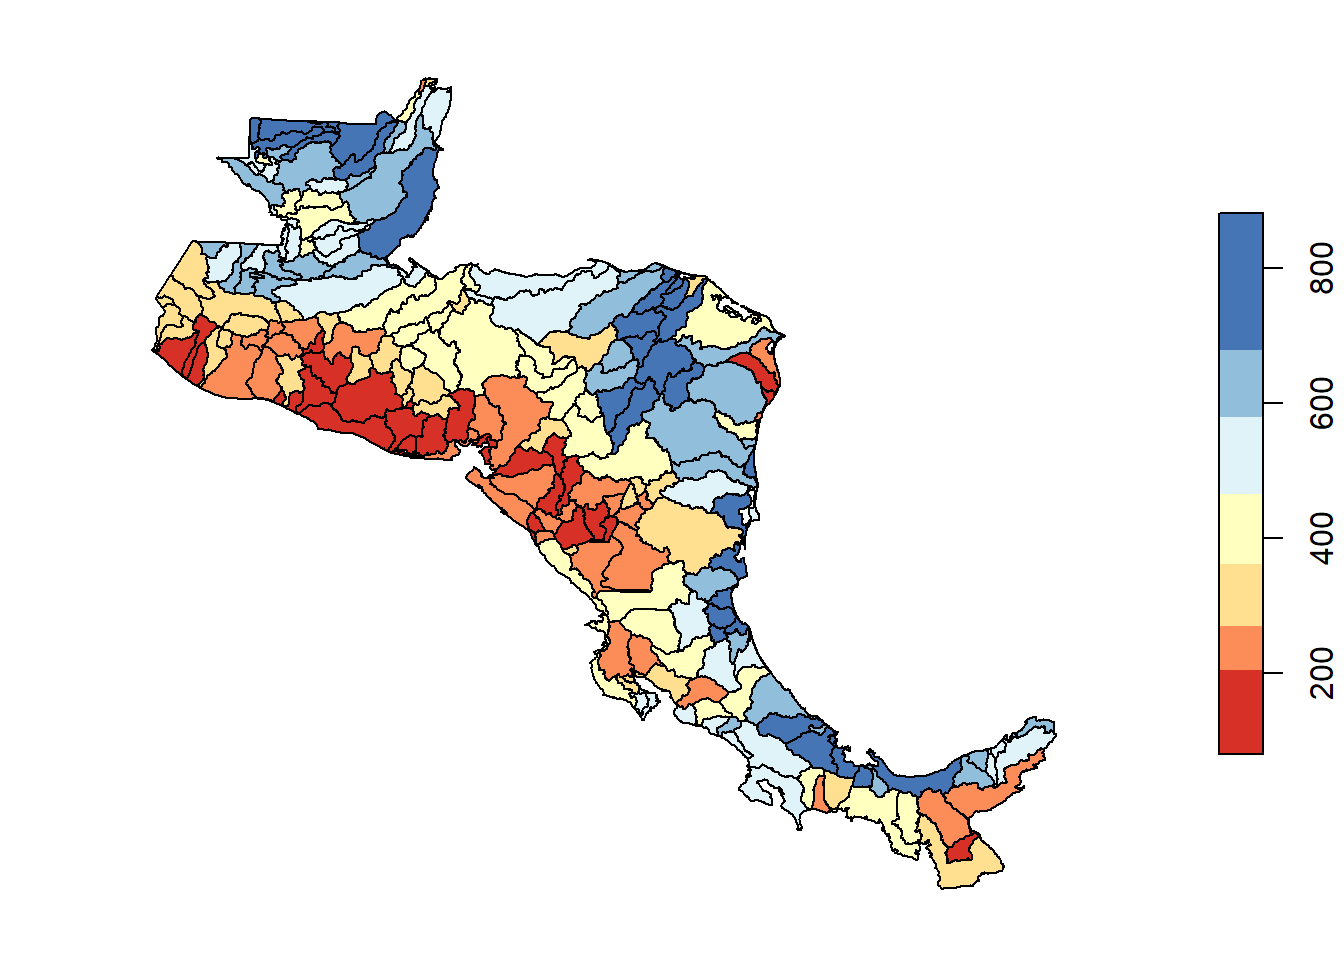
\includegraphics{bookdown-demo_files/figure-latex/unnamed-chunk-70-1.pdf}

\begin{Shaded}
\begin{Highlighting}[]
\FunctionTok{par}\NormalTok{(}\AttributeTok{mfrow=}\FunctionTok{c}\NormalTok{(}\DecValTok{1}\NormalTok{,}\DecValTok{1}\NormalTok{))}

\FunctionTok{plot}\NormalTok{(}\FunctionTok{st\_geometry}\NormalTok{(aoi\_test))}
\FunctionTok{plot}\NormalTok{(res,}\AttributeTok{add=}\NormalTok{T)}
\end{Highlighting}
\end{Shaded}

\includegraphics{bookdown-demo_files/figure-latex/unnamed-chunk-70-2.pdf}

\hypertarget{pitfalls}{%
\section{Pitfalls}\label{pitfalls}}

Brodie 2016 - multispecies map (connecting sicence policy and implementation for landscape scale connectivity) -\textgreater{} demonstrates that species do not all respond the same way to ``connectivity''

Corridor width -\textgreater{} buffer you use could influence the utility of the corridor (and does restoration reflect the proposed buffer for the corridor)

Animal behaviour - Migratory vs.~resident can influence the resistance surface

Large {[}Graph approach{]} vs.~small range \protect\hyperlink{circuitscape}{circuitscape} -\textgreater{}

\hypertarget{extentions}{%
\section{Extentions}\label{extentions}}

Climate connecitivy -\textgreater{} cooling benefit between ``connected'' areas -\textgreater{} the change in temperature between low and high locations = Resiliance.

Gray M, Micheli E, Comendant T, Merenlender A (2020) Quantifying climate-wise connectivity across a topographically diverse landscape. Land 9:1--18. \url{https://doi.org/10.3390/land9100355}

\begin{itemize}
\tightlist
\item
  Give it a quick go*?
\end{itemize}

  \bibliography{book.bib,packages.bib}

\end{document}
